\documentclass{article}
    \usepackage{amssymb}
    \usepackage[utf8]{inputenc}
    \usepackage[russian]{babel}
    \usepackage[left=2cm,right=2cm,
        top=2cm,bottom=2cm,bindingoffset=0cm]{geometry}
    \usepackage{hyperref}
    \hypersetup{
        colorlinks=true,
        linkcolor=blue,
        filecolor=magenta,      
        urlcolor=cyan,
    }
  \usepackage{graphicx}
  \graphicspath{{pictures/}}
  \DeclareGraphicsExtensions{.pdf,.png,.jpg}

\begin{document}
\begin{center}{\hugeОтчет по курсовой работе за неделю\\}\end{center}
Дата: 29.10.2020\\
Научные руководители: Герасимов С.В., Мещеряков А.В.\\
Студент: Немешаева Алиса\\
Курс: 4\\

\renewcommand{\labelitemi}{$\blacksquare$}
\renewcommand\labelitemii{$\square$}
\begin{enumerate}
    \item Найдена ошибка в генерации данных: в 37-ом пикселе из разбиения $n_{nside}=2$ healpix 
        содержался участок с очень большим по модулю значением, что приводило в определённых 
        ситуациях к превращения значения функции потерь в $NaN$.\\
    \item Создан новый алгоритм генерации данных для обучения - предыдущий использовал заранее 
        сгенерированные патчи, из-за чего использовал слишком много пространства на диске, новый 
        алгоритм генерирует данные прямо перед началом обучения, и требует почти в 10 раз меньше 
        данных, хранящихся на диске, что позволяет впоследствии перенести обучение на удалённые 
        сервера.\\
    \item На прошлой неделе было начато обучение новой модели, где в данные для обучения были 
        добавлены каталоги ACT. Было проведено тестирование для thr=0.1 (параметр порогового 
        значения маски) для модели на некоторых эпохах, чтобы оценить эффективность новой модели.\\

    \begin{figure}[h]
        \center{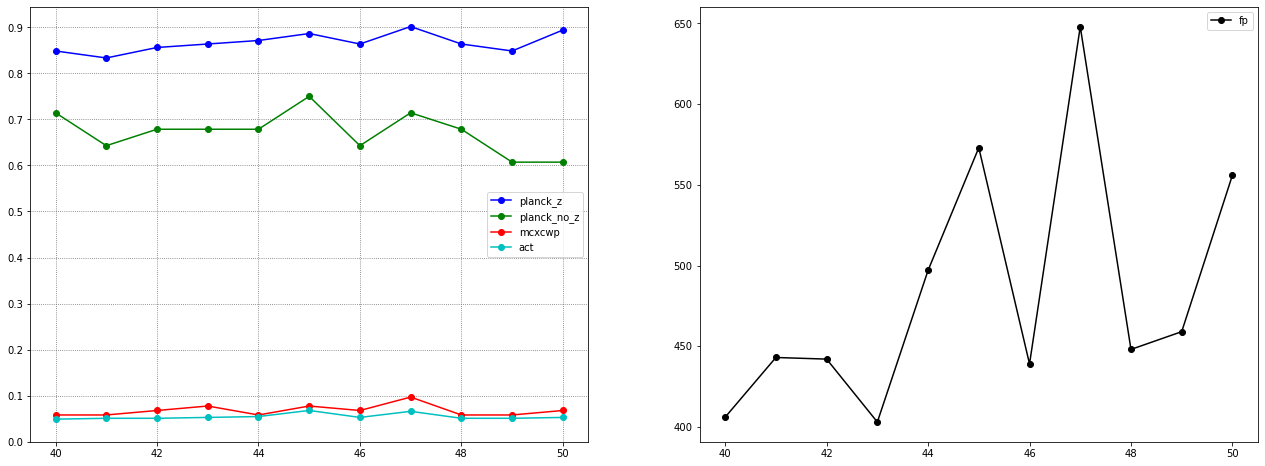
\includegraphics[width=0.6\linewidth]{ep40-50}}
        \caption{График recall для разных каталогов и график неизвестных объектов для эпох 40-50.}
    \end{figure}
    \begin{figure}[h]
        \center{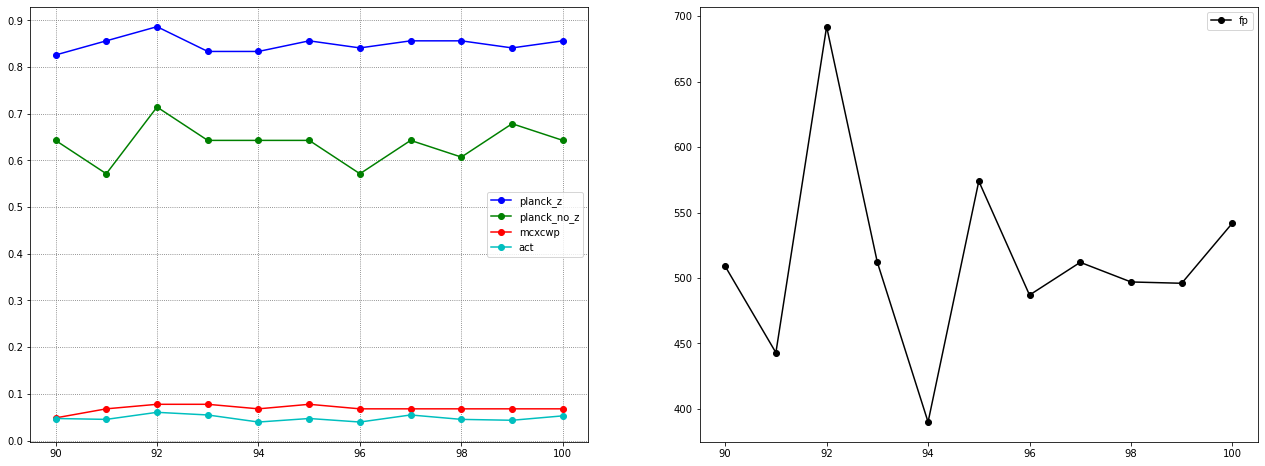
\includegraphics[width=0.6\linewidth]{ep90-100}}
        \caption{График recall для разных каталогов и график неизвестных объектов для эпох 90-100.}
    \end{figure}
    \item Каталоги planck\_z и act были в выборке для обучения, но recall на act очень низкий. Это 
        может быть связано с тем, что каталог ACT содержит данные только о некоторой части неба, 
        поэтому в большой части данных для обучения информации о скоплениях ACT не присутствует. \\
    \item Начато обучение новой модели только на тех областях, для которых существуют каталоги ACT.\\
\end{enumerate}

Отчет согласован с научным руководителем.\\
Общее количество строк кода за эту неделю: 344\\
\hyperlink{https://github.com/rt2122/data-segmentation-2}{Репозиторий}\\ 
\end{document}
